\documentclass[11pt,a4paper]{article}

\usepackage[utf8]{inputenc}
\usepackage[T1]{fontenc}
\usepackage[margin=2.5cm]{geometry}
\usepackage{booktabs}
\usepackage{array}
\usepackage{longtable}
\usepackage{xcolor}
\usepackage{amsmath}
\usepackage{graphicx}
\usepackage{placeins}
\usepackage[authoryear,round]{natbib}
\usepackage[colorlinks=true,linkcolor=black,citecolor=black,urlcolor=black]{hyperref}

\newcolumntype{L}[1]{>{\raggedright\arraybackslash}p{#1}}
\newcommand{\var}[1]{\texttt{#1}}

\title{Structure of Researchers' Views on Irreproducibility:\\
Principal Component Analysis and Regression of Survey Item Groups}
\date{}

\begin{document}
\maketitle

\begin{abstract}
\noindent
Six groups of ordinal survey items on reproducibility were analysed separately by principal component analysis (PCA) based on polychoric or Spearman correlations, with pairwise deletion of missing values and no imputation. The number of components was assessed by parallel analysis, and two components were rotated by varimax and by oblimin; the oblimin solution is the one used in the following steps. Parallel analysis suggested two components for one group (FACTORS) and one component for the other five. In three of those five (FIELD, DEM and CORE) the second eigenvalue lay 0.10--0.18 below the random-data benchmark, but the second component was interpretable and, in DEM and CORE, replicated in 97\% of 500 random split-half comparisons (88\% in FIELD, where it was less stable). The oblimin rotation showed that the two components are weakly to moderately correlated in five of the six groups ($r$ between 0.10 and 0.45). We therefore describe FACTORS, FIELD, DEM and CORE by two components. In the remaining two groups the second component is either a single item or rests on only three items, and we report them as one dimension plus a separate item.

\medskip\noindent
In a separate second step, the two oblimin components of CORE (recognition of the crisis and severity in one's own field) and their one-component summary were regressed on the component scores of the other groups and on respondent characteristics. The items were multiply imputed ($n=696$ in the main models; $n=393$ where NOREP is included), and complete-case models were fitted for comparison. The associations are small (about 0.1--0.2 SD per SD) and the explanatory power is low. Perceived flaws in the original research and both FIELD components (competitive field, visible and well-funded field) are positively related to all outcomes, author-level practices mainly to severity, and gender has opposite signs for recognition and severity. A Wald test did not reject equality of the effects of the two FIELD components for any outcome ($p$ between 0.22 and 0.94), so the data do not support a different role of the two components.
\end{abstract}

\section{Data and item groups}

The analysis uses $N=878$ respondents. The items were analysed in six thematic groups, each on its own. Missing values differ strongly between items (Table~\ref{tab:scales}), so each group uses all pairwise available observations and not only complete cases.

\begin{table}[ht]
\centering
\small
\begin{tabular}{@{}l c L{9.2cm}@{}}
\toprule
Group & Items & Content (item numbers refer to the questionnaire)\\
\midrule
FACTORS & 14 & Contribution of fourteen factors to irreproducibility (Q16), \var{fakt\_*}\\
NOREP & 3 & Failed replication experience: own experiment, someone else's experiment, own result not reproduced by others (Q18--20), yes/no\\
FREQ & 7 & Frequency of questionable research practices observed in one's field (Q23), \var{frek\_*}; \var{frek\_hacking} excluded (see below)\\
FIELD & 10 & Characteristics of one's field: funding, competition, pressure, media, field size, etc.\ (Q47--48), \var{obor\_*}\\
DEM & 6 & Respondent profile: gender, age, years in research, degree, citations, top-journal publication (Q38--43)\\
CORE & 5 & Reproducibility crisis: awareness, existence, estimated reproducible share, seriousness, increase (Q5--9)\\
\bottomrule
\end{tabular}
\caption{Item groups.}
\label{tab:groups}
\end{table}

\subsection{Response scales}

Table~\ref{tab:scales} gives the response scale of every item as coded in the analysis, the direction of the codes, and the number of valid answers. The labels were translated from Czech. Higher codes always mean more of what the item describes; where the questionnaire scale ran the other way (\var{rep\_podil}, \var{krize\_rep}, \var{obor\_vetsi}) the codes were reversed. For each group the table also gives the number of respondents with no missing item and the type of correlation used.

{\small
\begin{longtable}{@{}L{2.7cm} L{5.9cm} L{3.3cm} L{2.6cm}@{}}
\caption{Response scales as coded in the analysis, direction of the codes, and number of valid answers per item.}\label{tab:scales}\\
\toprule
Item & Scale (code = label) & Higher code means & Valid $N$\\
\midrule
\endfirsthead
\toprule
Item & Scale (code = label) & Higher code means & Valid $N$\\
\midrule
\endhead
\midrule
\multicolumn{4}{r}{\emph{continued on next page}}\\
\endfoot
\bottomrule
\endlastfoot
\multicolumn{4}{@{}l}{\textbf{FACTORS}: 14 items; 343 complete cases; polychoric correlations}\\
\var{fakt\_*} & 1 never, 2 rarely, 3 sometimes, 4 very often, 5 always & Factor contributes more often & 608--738\\
\addlinespace
\multicolumn{4}{@{}l}{\textbf{NOREP}: 3 items; 451 complete cases; polychoric correlations}\\
\var{nerep\_jaMuj}, \var{nerep\_jaCizi}, \var{nerep\_oniMuj} & 0 no, 1 yes (``I do not do experiments'' and ``I do not remember'' set to missing) & Failed replication experienced & 515--654\\
\addlinespace
\multicolumn{4}{@{}l}{\textbf{FREQ}: 7 items; 582 complete cases; Spearman correlations}\\
\var{frek\_*} & 0, 10, 20, \dots, 100 (coded 1--11) & Practice observed more often & 760--818\\
\addlinespace
\multicolumn{4}{@{}l}{\textbf{FIELD}: 10 items; 878 complete cases; polychoric correlations}\\
\var{obor\_*} except \var{obor\_tlak} & 1 definitely not, 2 rather not, 3 don't know, 4 rather yes, 5 definitely yes & Field has the characteristic to a greater degree & 878\\
\var{obor\_tlak} & 1 no (definitely or rather not), 2 don't know, 3 rather yes, 4 definitely yes & Field has the characteristic to a greater degree & 878\\
\addlinespace
\multicolumn{4}{@{}l}{\textbf{CORE}: 5 items; 700 complete cases; Spearman correlations}\\
\var{rep\_type} & 0 no, 1 yes & Has heard of the crisis & 806\\
\var{krize\_rep} & 1 no crisis, 2 don't know, 3 yes, insignificant crisis, 4 yes, significant crisis & Crisis judged more serious & 804\\
\var{rep\_podil} & 1 = 100\%, 2 = 90\%, \dots, 11 = 0\% (estimated share of reproducible results) & Smaller share reproducible (scale reversed) & 718\\
\var{nerep\_problem}, \var{nerep\_narust} & 1 strongly disagree, 2 somewhat disagree, 3 neutral, 4 somewhat agree, 5 strongly agree & Stronger agreement & 790, 786\\
\addlinespace
\multicolumn{4}{@{}l}{\textbf{DEM}: 6 items; 873 complete cases; polychoric correlations}\\
\var{gender} & 0 man, 1 woman (``other'' set to missing) & Woman & 873\\
\var{vek} & 1 = 18--34, 2 = 35--44, 3 = 45--54, 4 = 55--64, 5 = 65 and more & Older & 878\\
\var{kar\_praxe} & 1 less than 5 years, 2 = 5--9, 3 = 10--19, 4 = 20 and more & More years in research & 878\\
\var{kar\_titul} & 1 Bc./Mgr./Ing., 2 CSc./Ph.D., 3 associate professor (Docent), 4 DrSc./DSc., 5 professor & Higher degree & 878\\
\var{kar\_citace} & 1 up to 100, 2 up to 500, 3 up to 1000, 4 up to 5000, 5 more & More citations & 878\\
\var{kar\_nejlepsi} & 1 no, 2 yes & Published in a top journal & 878\\
\end{longtable}
}


\paragraph{Exclusions.}
Free-text items and the nominal variable giving the Academy of Sciences category (\var{kar\_kategorie}) were not included. The item \var{frek\_hacking} (p-hacking) has 494 missing values out of 878 (56\%) and was left out of FREQ. Including it reduced the number of respondents with complete data in that group from 582 to 322 and did not change the number of retained components.

\paragraph{Recoding of CORE.}
All CORE items were coded so that higher values mean a greater problem with reproducibility. For \var{krize\_rep} the four answers were ordered as: no crisis (1), don't know (2), insignificant crisis (3), significant crisis (4). Treating ``don't know'' as a point between ``no crisis'' and ``insignificant crisis'', and not as missing, is supported by two observations. First, among respondents who had not heard of the reproducibility crisis, the ratio of those unaware to those aware was almost identical for ``don't know'' (141/77 $\approx$ 1.83) and ``no crisis'' (60/33 $\approx$ 1.82), and much lower for the two ``yes'' answers. Second, the mean ratings of three related items changed monotonically along the four categories, with ``don't know'' lying between ``insignificant crisis'' and ``no crisis'' (Table~\ref{tab:dontknow}).

\begin{table}[ht]
\centering
\small
\begin{tabular}{@{}l c c c@{}}
\toprule
\var{krize\_rep} & \var{rep\_podil} & \var{nerep\_problem} & \var{nerep\_narust}\\
\midrule
Yes, significant crisis   & 6.76 & 3.82 & 3.62\\
Yes, insignificant crisis & 7.91 & 2.83 & 3.13\\
Don't know                & 8.20 & 2.59 & 2.88\\
No crisis                 & 8.79 & 2.02 & 2.52\\
\bottomrule
\end{tabular}
\caption{Mean ratings of three related items by answer to \var{krize\_rep}. The table was computed before \var{rep\_podil} was reversed, so for \var{rep\_podil} a higher code means a larger estimated share of reproducible results; for the other two items a higher code means stronger agreement.}
\label{tab:dontknow}
\end{table}

\paragraph{Coding of DEM.}
Gender was coded as binary (0 = man, 1 = woman); five respondents who chose ``other'' were set to missing because the group was too small for analysis. Top-journal publication was coded 1 = no, 2 = yes. Age was coded in five bands (1 = 18--34, \dots, 5 = 65 and more) and the academic degree in five ordered categories (1 = Bc./Mgr./Ing., 2 = CSc./Ph.D., 3 = associate professor, 4 = DrSc./DSc., 5 = professor); all codes 1--5 occur in the data. All other items were ordered from low to high.

\paragraph{Coding of FIELD.}
All FIELD items were answered by all 878 respondents. For \var{obor\_tlak} the two negative answers (definitely not, rather not) form one category (1), followed by ``don't know'' (2), ``rather yes'' (3) and ``definitely yes'' (4), so this item has four categories and the other nine have five.

\section{Principal component analysis: methods}

\paragraph{Correlations.}
For each group, a correlation matrix of the integer-coded items was computed with pairwise deletion of missing values. Polychoric correlations were used (tetrachoric for binary items). For groups containing an item with more than eight categories (FREQ and CORE, with 11-point items) polychoric correlations are not appropriate, and Spearman correlations were used instead. The matrix was smoothed to the nearest positive definite matrix when needed. Results for groups based on different correlation types are therefore not strictly comparable.

\paragraph{PCA.}
PCA was computed from the eigendecomposition of the correlation matrix, so that all items are standardised. The sign of each component was fixed so that its largest absolute loading is positive. Component scores are defined only for respondents with no missing item in the group.

\paragraph{Number of components.}
The number of components was assessed by parallel analysis \citep{horn1965}, which compares the observed eigenvalues with the mean eigenvalues of 500 random data sets of the same size (fixed random seed), retaining components while the observed eigenvalue exceeds the random one. The sample size used for the random data was the number of respondents with complete data in the group, but not less than $N/2=439$; this lower bound applies only to FACTORS (343 complete cases). The Kaiser criterion (eigenvalue $>1$) was not used, because it is known to retain too many components \citep{zwick1986}. A cumulative-variance threshold was also rejected: 90\% of the variance required 12 of 14 components in FACTORS, 8 of 10 in FIELD and 6 of 7 in FREQ, since the items are only moderately correlated.

\paragraph{Rotation.}
Two components were rotated by varimax to obtain a simple structure in which each item loads mainly on one component. Rotation changes how the explained variance is divided between the components, but not the total explained by the two. An oblique rotation (oblimin) of the same correlation matrix was computed as well, which allows the two components to be correlated; the correlation between them is reported in Section~\ref{sec:phi}. Because the oblimin solution is used in the following steps of the analysis, its pattern loadings are plotted in Appendix~\ref{app:fig} and listed next to the varimax loadings in Appendix~\ref{app:load}. With correlated components the per-component variance shares overlap and are not additive, so the total variance explained is taken from the unrotated solution.

\paragraph{Split-half stability.}
The respondents were randomly split into two halves 500 times. In each split the two-component varimax solution was computed in both halves, and the loadings were compared using Tucker's congruence coefficient, matching the components between halves (axes may swap) and ignoring sign. Values of 0.85--0.94 are conventionally read as fair similarity and 0.95 or more as equality of components \citep{lorenzo2006}. Comparing the halves with each other, and not with the full sample, avoids overlap between the compared solutions.

\section{Principal component analysis: results}

\subsection{Summary}

Table~\ref{tab:summary} gives the retention results and Table~\ref{tab:dims} the interpretation of the rotated components. The percentages of variance are for the two components together; the first three eigenvalues of every group, observed and random, are in Appendix~\ref{app:eig} and all loadings in Appendix~\ref{app:load}.

\begin{table}[ht]
\centering
\small
\begin{tabular}{@{}l c c c c L{4.6cm}@{}}
\toprule
Group & Items & \shortstack{Parallel\\analysis} & \shortstack{2nd eigenvalue\\(obs.\ / random)} & \shortstack{Variance,\\2 comp.} & Evidence for a second dimension\\
\midrule
FACTORS & 14 & 2 & 1.62 / 1.24 & 34.8\% & Strong\\
FIELD   & 10 & 1 & 1.02 / 1.12 & 50.3\% & Moderate: second eigenvalue below the benchmark, clear content, second axis less stable in split-halves\\
DEM     & 6 & 1 & 0.93 / 1.06 & 77.0\% & Moderate: second axis dominated by gender and top-journal publication\\
CORE    & 5 & 1 & 0.87 / 1.05 & 67.6\% & Moderate: weak eigenvalue, content follows item wording\\
FREQ    & 7 & 1 & 0.85 / 1.09 & 64.9\% & Weak: second axis is a single item\\
NOREP   & 3 & 1 & 0.43 / 1.00 & 87.9\% & Weak: only three items, unstable\\
\bottomrule
\end{tabular}
\caption{Number of components and strength of the evidence for a second dimension.}
\label{tab:summary}
\end{table}

\begin{table}[ht]
\centering
\small
\begin{tabular}{@{}l L{5.8cm} L{5.8cm}@{}}
\toprule
Group & RC1 & RC2\\
\midrule
FACTORS & Flaws in the original research: misconduct, weak oversight and review, selective reporting, withheld data and code & Intrinsic difficulty: bad luck, reagent variability, methods requiring special expertise, errors by replicators\\[4pt]
FIELD & Hyper-competitive, fast-growing field: pressure for results, publication growth, competition, rapid obsolescence, complexity; influx of researchers loads on both components, more on RC1 & Visible, publicly funded field: public opinion, media exposure, subsidies, field size\\[4pt]
DEM & Seniority: age, years in research, degree, citations & Gender and publication success: male gender, top-journal publication and, less strongly, citations\\[4pt]
CORE & General recognition of the crisis: awareness, belief that it exists, increase during the career & Severity of the problem in one's own field: estimated reproducible share, seriousness\\[4pt]
FREQ & Author-level practices: overselling, unjustified generalisation, trendy methods, buzzwords, pointless studies, salami slicing & \var{frek\_positiv} (publication of positive results only) alone\\[4pt]
NOREP & Others failing to reproduce my results & Me failing to reproduce others' work; failing to reproduce my own loads on both\\
\bottomrule
\end{tabular}
\caption{Interpretation of the varimax-rotated components.}
\label{tab:dims}
\end{table}

\subsection{Correlation between components}
\label{sec:phi}

Table~\ref{tab:phi} gives the correlation between the two components after oblique rotation. A correlation of about 0.32 or more (10\% shared variance) is commonly taken as a reason to prefer an oblique solution \citep{tabachnick2013}.

\begin{table}[ht]
\centering
\small
\begin{tabular}{@{}l c c L{6.2cm}@{}}
\toprule
Group & Correlation & Shared variance & Reading\\
\midrule
FACTORS & 0.10 & 1\%  & Essentially independent; varimax is fully justified\\
FIELD   & 0.45 & 20\%  & Moderate to high: related but distinct\\
CORE    & 0.35 & 13\%  & Moderate\\
DEM     & 0.44 & 19\%  & Moderate to high: seniority is related to the gender and top-journal component\\
FREQ    & 0.34 & 11\%  & Moderate; the second component is a single item\\
NOREP   & 0.58 & 34\%  & High: supports a single dimension\\
\bottomrule
\end{tabular}
\caption{Correlation between the two components after oblimin rotation.}
\label{tab:phi}
\end{table}

With the exception of NOREP, the correlations lie between 0.10 and 0.45, so the second components are related to the first but carry largely their own information. The oblique loadings assign the items to the same components as varimax in all six groups (Appendix~\ref{app:load}), and the pattern loadings are plotted in Figures~\ref{fig:obl-FACTORS}--\ref{fig:obl-NOREP} (Appendix~\ref{app:fig}). In FREQ the second component is the single item \var{frek\_positiv} (loading 0.96), and in NOREP the two components are essentially the single items \var{nerep\_oniMuj} (0.99) and \var{nerep\_jaCizi} (0.98), with \var{nerep\_jaMuj} between them. Such components are individual items, not dimensions, and for NOREP the correlation of 0.58 mainly describes how strongly these two items are related.

\subsection{Interpretation by group}

\paragraph{FACTORS.} The first component (22.3\%) collects explanations that blame the original research and the system around it: fraud, selective reporting, withheld data and protocols, insufficient supervision and peer review, career pressure, poor design and weak statistics. The second (12.6\%) collects explanations that do not blame the original authors: bad luck, reagent variability, methods needing special expertise, and errors by those who replicate. Replicator errors and poor design load on both components. Parallel analysis supports two components, and the near-zero correlation between the components (0.10) shows that the two kinds of explanation are almost independent.

\paragraph{FIELD.} The first component (27.6\%) describes a competitive, fast-growing field with strong pressure on results. The rapid influx of researchers loads on both components (varimax 0.59 and 0.46) but mainly on the first in the oblique solution (0.54 and 0.32). The second component (22.7\%) describes a field in the public eye, with media exposure, influence of public opinion, and high funding. Its content is clear, but its statistical support is weaker than in FACTORS: the second eigenvalue is 0.10 below the random benchmark (1.02 against 1.12), it is close to the third eigenvalue (0.92), and the second component was less stable in the split-half check than those of DEM and CORE (see below).

\paragraph{DEM.} The first component (51.5\%) is seniority. The second (25.4\%) is defined by gender and top-journal publication and, less strongly, citations. The loading of gender is negative because women are coded 1, so the component expresses male gender: in this sample men are more often top-journal authors and, to a lesser degree, more often highly cited. Gender also correlates with the seniority component (about $-0.34$ in the oblique structure matrix, women being less senior), so the gender gap is partly a seniority effect. The second eigenvalue is 0.13 below the random benchmark (0.93 against 1.06). The component is dominated by two binary items, and we report it as an association between these items and citations, not as a latent construct.

\paragraph{CORE.} After recoding so that higher values always mean a greater problem, all loadings are positive. The first component (35.5\%) is general recognition of the crisis (awareness, belief that it exists, increase during the career). The second (32.1\%) is the assessment of the problem in the respondent's own field (estimated reproducible share, seriousness). The distinction follows the wording of the questions, which is stronger support than the eigenvalue pattern, where the second eigenvalue (0.87) lies clearly below the random benchmark (1.05).

\paragraph{FREQ.} All practices except one load on the first component (47.6\%). The second (17.3\%) is the single item \var{frek\_positiv}, which means that this item is weakly related to the others. We interpret this as perceived publication bias being separate from author-level practices, and report it as an item, not as a dimension.

\paragraph{NOREP.} Three binary items give a two-component solution (46.8\% and 41.1\% after rotation) that follows the roles of the respondent (being replicated or replicating). With three items such a split is almost guaranteed, and the second eigenvalue is far below the random benchmark (0.43 against 1.00). In the oblique solution the two components are almost single items (loadings 0.98--0.99) correlated at 0.58. We do not treat it as evidence of two dimensions.

\subsection{Split-half stability}

Table~\ref{tab:split} shows the stability of the two varimax components in random split-half comparisons.

\begin{table}[ht]
\centering
\small
\begin{tabular}{@{}l c c c c c c@{}}
\toprule
 & \multicolumn{3}{c}{RC1} & \multicolumn{3}{c}{RC2}\\
\cmidrule(lr){2-4}\cmidrule(lr){5-7}
Group & Median & 2.5\% quantile & Splits $\geq 0.85$ & Median & 2.5\% quantile & Splits $\geq 0.85$\\
\midrule
FACTORS & \multicolumn{6}{c}{not available (computation failed in all 500 splits; to be added)}\\
FIELD  & 0.95 & 0.77 & 92\% & 0.93 & 0.42 & 88\%\\
CORE   & 0.97 & 0.85 & 98\% & 0.97 & 0.83 & 97\%\\
DEM    & 1.00 & 0.97 & 100\% & 0.98 & 0.81 & 97\%\\
FREQ   & 1.00 & 0.99 & 100\% & 0.95 & 0.84 & 97\%\\
NOREP  & 0.90 & 0.81 & 92\% & 0.90 & 0.54 & 85\%\\
\bottomrule
\end{tabular}
\caption{Split-half congruence (Tucker's coefficient) of the varimax components in 500 random splits. No split failed in the groups shown; ``Splits $\geq 0.85$'' is the share of splits in which the congruence reached 0.85.}
\label{tab:split}
\end{table}

In DEM and CORE the median congruence is 0.97--1.00 for RC1 and 0.97--0.98 for RC2, and the second component reaches 0.85 in 97\% of the splits (2.5\% quantile 0.81 in DEM and 0.83 in CORE). FIELD is less stable: the medians are 0.95 (RC1) and 0.93 (RC2), but the second component falls below 0.85 in 12\% of the splits and its 2.5\% quantile is 0.42, so in some halves the second varimax axis of FIELD is not recovered. A possible reason is that the second and third eigenvalues of FIELD are close (1.02 and 0.92), so that a third component can enter the plane of the first two in some halves. The second component of FREQ, which is a single item, is also stable (median 0.95), so stability alone does not make a component a dimension. NOREP has the lowest typical congruence (median 0.90 for both components, 85\% of the splits at or above 0.85 for RC2, 2.5\% quantile 0.54), which agrees with treating its second component as an artefact of having only three items. Each half contains only half of the respondents, so these values understate the stability of the full-sample solutions. The medians of RC1 and RC2 are similar because two orthogonal varimax axes in one plane rotate together, whereas the lower tails differ more (FIELD, NOREP). The check therefore supports the stability of the two-dimensional solution as a whole more than that of the second axis separately.

\section{Regression of the CORE components on the other groups}
\label{sec:reg}

This section relates the two CORE components to the components of the other item groups. The aim is descriptive: to see which views and respondent characteristics go together with recognising the reproducibility crisis and with judging its severity in one's own field. The associations are not causal and the analysis is exploratory.

\subsection{Design}

\paragraph{Outcomes.}
The outcomes are the two oblimin components of CORE, COR1 (recognition of the crisis) and COR2 (severity in one's own field). Because parallel analysis retained one component for CORE, the first unrotated component COR0 is analysed as well, so that the one- and the two-component description are both reported. All three scores are oriented so that higher values mean a greater problem with reproducibility.

\paragraph{Predictors.}
The predictors are scores of the other groups: the two oblimin components of FACTORS (\var{FAC1}, flaws in the original research; \var{FAC2}, intrinsic difficulty) and of FIELD (\var{FLD1}, competitive field; \var{FLD2}, visible and well-funded field), the first FREQ component (\var{FRQ1}, author-level practices) together with the single item \var{frek\_positiv}, the seniority component of DEM (\var{DEM1}) with gender and top-journal publication as single variables, and for NOREP the first component (\var{NOR1}) with the item \var{nerep\_jaCizi}. The weights of every score were fixed from the oblimin solutions of Section~\ref{sec:phi} and Appendix~\ref{app:load}, so that numbering and signs agree with the rest of the report. Scores are computed from the standardised items and standardised to mean 0 and standard deviation 1; \var{frek\_positiv} is standardised as well, while gender (1 = woman) and top-journal publication are binary 0/1 variables. Coefficients of score predictors are therefore changes of the outcome in SD units per SD of the predictor, and coefficients of binary predictors are differences between the two groups in SD units of the outcome.

\paragraph{Models.}
Two sets of linear models were fitted by ordinary least squares with HC3 standard errors \citep{long2000}. Block-wise models use one predictor group at a time, with and without adjustment for DEM, on the original data. Joint models contain all groups at once. For the joint models the items of FACTORS, FIELD, FREQ, DEM and CORE were multiply imputed (predictive mean matching, 20 data sets, 10 iterations; \citealp{vanbuuren2011}), the scores were recomputed in every imputed data set, and respondents whose outcome was originally missing were dropped after imputation \citep{vonhippel2007}. Estimates were pooled by Rubin's rules with the Barnard--Rubin degrees of freedom \citep{rubin1987,barnard1999}. NOREP was not imputed, because the answers ``I do not do experiments'' and ``I do not remember'' are structurally missing; models containing NOREP therefore use the 393 respondents with observed NOREP items. Four respondents who answered ``other'' for gender are excluded from the joint models, which gives $n=696$. For comparison, the joint models were also fitted on the 245 complete cases. As a robustness check, the five CORE items were analysed one by one (logistic regression for \var{rep\_type}, proportional-odds models for the ordinal items), and a variant with ``don't know'' of \var{krize\_rep} set to missing was added.

\paragraph{Comparing the two FIELD components.}
The hypothesis $H_0\colon \beta_{\mathrm{FLD1}}=\beta_{\mathrm{FLD2}}$ was tested separately for each outcome by a Wald test of the contrast $\beta_{\mathrm{FLD1}}-\beta_{\mathrm{FLD2}}$. The variance of the contrast uses the full covariance matrix of the estimates, including the covariance of the two coefficients. In the imputed data the contrast and its variance were computed in every data set and pooled by Rubin's rules, and the Wald statistic is the squared pooled $t$ statistic ($F$ on 1 and $\nu$ degrees of freedom). The test is meaningful because both scores are in SD units, but it compares partial effects of two correlated components ($r=0.45$, Table~\ref{tab:phi}).

\subsection{Results}

All effects are small, about 0.1--0.2 SD of the outcome per SD of the predictor, and the explanatory power is low. Each predictor group alone explains at most 12\% of the variance of an outcome (15\% after adjustment for DEM), and in the complete-case joint models $R^2$ is 0.09--0.21 ($n=245$, so this is optimistic). Adjusting the block-wise models for DEM changes the estimates only slightly, so demographics do not confound the effects of the other groups. Table~\ref{tab:reg-joint} gives the joint models with multiple imputation.

\begin{table}[ht]
\centering
\small
\begin{tabular}{@{}l L{3.6cm} >{\centering\arraybackslash}p{2.5cm} >{\centering\arraybackslash}p{2.5cm} >{\centering\arraybackslash}p{2.5cm}@{}}
\toprule
Predictor & Meaning & COR1 (recognition) & COR2 (severity in own field) & COR0 (one component)\\
\midrule
\var{FAC1} & Flaws in original research & 0.16*** (0.038) & 0.16*** (0.037) & 0.20*** (0.038) \\
\var{FAC2} & Intrinsic difficulty & 0.00 (0.036) & $-$0.07* (0.034) & $-$0.04 (0.035) \\
\var{FLD1} & Competitive field & 0.17*** (0.040) & 0.10* (0.041) & 0.16*** (0.040) \\
\var{FLD2} & Visible, funded field & 0.09* (0.040) & 0.16*** (0.040) & 0.15*** (0.039) \\
\var{FRQ1} & Author-level practices & 0.08 (0.044) & 0.21*** (0.044) & 0.17*** (0.043) \\
\var{frek\_positiv} & Perceived publication bias & 0.04 (0.043) & 0.09* (0.044) & 0.08 (0.043) \\
\var{DEM1} & Seniority & 0.01 (0.039) & $-$0.05 (0.038) & $-$0.02 (0.038) \\
\var{gender} & Gender (1 = woman) & $-$0.17* (0.079) & 0.19* (0.075) & 0.01 (0.075) \\
\var{top\_journal} & Top-journal author & $-$0.07 (0.085) & $-$0.19* (0.080) & $-$0.16 (0.082) \\
\addlinespace
\var{FLD0} & FIELD as one component$^{a}$ & 0.22*** (0.035) & 0.21*** (0.038) & 0.26*** (0.036)\\
\bottomrule
\end{tabular}
\caption{Joint linear models with multiple imputation, $n=696$: coefficient (pooled HC3 standard error). Standardised predictors, except gender and top-journal publication (0/1). $^{*}p<0.05$, $^{**}p<0.01$, $^{***}p<0.001$. $^{a}$ Separate model in which \var{FLD1} and \var{FLD2} are replaced by the first unrotated FIELD component.}
\label{tab:reg-joint}
\end{table}

\paragraph{Most stable effects.}
\var{FAC1}, \var{FLD1} and \var{FLD2} are positive for all three outcomes, and \var{FRQ1} is positive mainly for COR2 (0.21, against 0.08 for COR1, $p=0.063$). A one-component FIELD score is clearly positive for all outcomes (0.21--0.26, $p<0.001$), so the FIELD result does not depend on the less stable second component. In the complete cases the direction of \var{FLD1}, \var{FRQ1} (on COR2), gender and top-journal publication agrees with the imputed models, whereas \var{FLD2} is weaker (0.06--0.08, not significant), \var{FAC2} changes its sign for COR2, and \var{FAC1} on COR1 falls to 0.08 (standard error 0.065), which is within sampling error of the imputed estimate of 0.16. The small effect of \var{FAC2} on COR2 ($-0.07$, $p=0.036$) should therefore not be interpreted.

\paragraph{Why two components help.}
Gender has opposite signs for COR1 ($-0.17$) and COR2 ($+0.19$) and cancels in COR0 (0.01). \var{FAC2} and \var{FRQ1} also act mainly on COR2. A single CORE dimension would hide these differences, which supports reporting both descriptions.

\paragraph{Gender.}
The effect on COR2 is supported at item level: women estimate a smaller share of reproducible results (\var{rep\_podil}, odds ratio 1.47, 95\% CI 1.10--1.95) and rate the problem as more serious (\var{nerep\_problem}, odds ratio 1.37, 1.03--1.81). The effect on COR1 is not, since none of its items is significant on its own, and it should be treated as fragile.

\paragraph{Seniority.}
\var{DEM1} is null for the components but not for single items. Seniority raises agreement that irreproducibility has increased during one's career (\var{nerep\_narust}, odds ratio 1.27, $p=0.001$), which is partly mechanical because of the length of a career, and it lowers the odds of calling the crisis significant among respondents with an opinion (\var{krize\_rep} without ``don't know'', odds ratio 0.76, $p=0.001$). These opposite effects cancel in the components.

\paragraph{NOREP.}
In the 393 respondents with observed NOREP items, \var{NOR1} is related to recognition (COR1: 0.17, $p=0.032$; COR0: 0.14, $p=0.055$) but not to severity (COR2: 0.06, $p=0.41$). The variance inflation factors of \var{NOR1} and \var{nerep\_jaCizi} are about 2.5, so their separate effects cannot be identified. The top-journal effect is larger in this subsample (COR2: $-0.33$, $p=0.001$), but these respondents are a selected group who do experiments.

\subsection{FLD1 compared with FLD2}
\label{sec:wald}

The point estimates suggest that \var{FLD1} matters somewhat more for recognition and \var{FLD2} for severity in one's own field (Table~\ref{tab:reg-joint}). Table~\ref{tab:wald} tests whether the two coefficients differ.

\begin{table}[ht]
\centering
\small
\begin{tabular}{@{}l l r c c c c c c@{}}
\toprule
Model & Outcome & $n$ & \var{FLD1} & \var{FLD2} & Difference & SE & $F$ & $p$\\
\midrule
MI, all respondents & COR1 & 696 & 0.17 & 0.09 & 0.08 & 0.068 & 1.28 & 0.259 \\
 & COR2 & 696 & 0.10 & 0.16 & $-$0.06 & 0.068 & 0.88 & 0.348 \\
 & COR0 & 696 & 0.16 & 0.15 & 0.01 & 0.066 & 0.04 & 0.845 \\
\addlinespace
MI, observed NOREP & COR1 & 393 & 0.12 & 0.11 & 0.01 & 0.094 & 0.00 & 0.944 \\
 & COR2 & 393 & 0.10 & 0.14 & $-$0.03 & 0.091 & 0.14 & 0.708 \\
 & COR0 & 393 & 0.13 & 0.15 & $-$0.02 & 0.094 & 0.03 & 0.871 \\
\addlinespace
Complete cases & COR1 & 245 & 0.19 & 0.07 & 0.13 & 0.125 & 1.00 & 0.317 \\
 & COR2 & 245 & 0.17 & 0.06 & 0.11 & 0.120 & 0.82 & 0.365 \\
 & COR0 & 245 & 0.22 & 0.08 & 0.14 & 0.116 & 1.53 & 0.217 \\
\bottomrule
\end{tabular}
\caption{Wald test of $\beta_{\mathrm{FLD1}}=\beta_{\mathrm{FLD2}}$ per outcome (difference = \var{FLD1} $-$ \var{FLD2}; SE of the difference from the full covariance matrix of the estimates; $F$ on 1 and $\nu$ degrees of freedom).}
\label{tab:wald}
\end{table}

The hypothesis of equal effects is not rejected for any outcome in any of the three settings ($p$ between 0.22 and 0.94). In the imputed models with all respondents the differences are 0.08 for COR1 ($p=0.26$) and $-0.06$ for COR2 ($p=0.35$), and close to zero for COR0 ($p=0.85$), which is the expected result when the two components differ only in emphasis. The same holds in the block-wise models, where the largest difference is for COR1 (0.125, $p=0.071$; 0.123, $p=0.079$ after adjustment for DEM) and all other $p$ values are 0.24 or more. The standard error of a difference is about 0.07 (0.09 in the NOREP subsample), so a difference would have to exceed about 0.13 SD to be significant, and a non-significant test is not evidence that the two effects are equal. The data therefore show that both FIELD components go together with a more serious view of the crisis, but they do not allow one to claim that the two components relate differently to recognition and to severity. This agrees with the one-component FIELD score being sufficient (Table~\ref{tab:reg-joint}) and with the weaker split-half stability of the second FIELD component. The COR1/COR2 contrasts for the other predictors, for example gender, come from separate models and have not been tested formally.

\subsection{Cautions}

\begin{itemize}
\item The proportional-odds assumption of the item-level models is clearly violated for \var{DEM1} and top-journal publication (on \var{krize\_rep}, \var{nerep\_narust} and \var{nerep\_problem}) and for \var{FAC1} on \var{rep\_podil}. These odds ratios are average effects over the thresholds only.
\item FACTORS, FIELD and FREQ are all perceptions of the same respondent, so part of their association with severity may be a general tendency to rate things as bad.
\item No adjustment for multiplicity was made; findings with $p$ between 0.01 and 0.05 are exploratory.
\item The differences between components other than the tested \var{FLD1}--\var{FLD2} contrast are descriptive, and the split of FIELD into two components was the least stable one in the split-half check.
\end{itemize}

\section{Conclusion}

\subsection{Principal component analysis}

\begin{enumerate}
\item \textbf{FACTORS.} Two components are supported by parallel analysis, interpretability and structure. Respondents distinguish attributing irreproducibility to flaws in the original research and its system from attributing it to intrinsic difficulty and chance, and the two views are almost uncorrelated ($r=0.10$).
\item \textbf{FIELD, CORE and DEM.} Parallel analysis suggested one component, and the second eigenvalue was below the random benchmark by 0.10 (FIELD), 0.13 (DEM) and 0.18 (CORE). We retain two components because the rotated solutions are interpretable and follow the content of the items, and in DEM and CORE the second component recurs in 97\% of random split-half comparisons; the components are moderately correlated ($r=0.35$--$0.45$). The support is weakest for FIELD, where the second component was recovered in 88\% of the splits only (2.5\% quantile 0.42). Because retaining too few components is generally regarded as the more serious error \citep{fabrigar1999}, and interpretability is a recognised criterion in addition to the eigenvalue rule, we regard this as a justified departure from the parallel-analysis count. In DEM, the second component is dominated by two binary items (gender and top-journal publication) and citations, and in CORE its support rests largely on the wording of the questions.
\item \textbf{FREQ and NOREP.} The evidence for a second dimension is weak. We describe FREQ by one general component plus the separate item \var{frek\_positiv}, and NOREP by one component with the three items reported individually. The oblique solutions confirm that the second component of FREQ, and both components of NOREP, are essentially single items (loadings 0.96--0.99), and the split-half check shows that the NOREP solution has the lowest typical stability (median congruence 0.90).
\item \textbf{General.} Between 35\% and 88\% of the variance is explained by two components, depending on the group, and the share is low where items are only moderately correlated (FACTORS). The components are summaries of the items, not measured constructs, and for FIELD, DEM and CORE, where the second eigenvalue lies below the random benchmark, both the one-component and the two-component description should be reported.
\end{enumerate}

\subsection{Regression}

\begin{enumerate}
\item \textbf{Size of the effects.} The associations of the CORE components with the other groups are small, about 0.1--0.2 SD of the outcome per SD of the predictor. A single predictor group explains at most 12\% of the variance of an outcome (15\% after adjustment for DEM), and the complete-case joint models explain 9--21\% ($n=245$, so this is optimistic).
\item \textbf{Most stable associations.} Perceived flaws in the original research (\var{FAC1}) and both FIELD components (\var{FLD1}, \var{FLD2}) are positively related to all three outcomes, and author-level practices (\var{FRQ1}) mainly to severity in one's own field (COR2). A one-component FIELD score is clearly positive for all outcomes (0.21--0.26), so this result does not depend on the less stable second FIELD component.
\item \textbf{FLD1 and FLD2.} The Wald test does not reject equality of the two FIELD effects for any outcome (joint models: $p$ between 0.22 and 0.94). The point estimates lean towards \var{FLD1} for recognition and \var{FLD2} for severity, but the power to detect a difference of this size is low, so the data neither show nor exclude a different role of the two components.
\item \textbf{Why two outcome components are reported.} Gender has opposite signs for recognition ($-0.17$) and severity ($+0.19$) and cancels in the one-component score, and seniority has opposite item-level effects that cancel in the components. The gender effect on severity is supported at item level, the one on recognition is not. The differences between COR1 and COR2 are descriptive; only the FLD1--FLD2 contrast was tested formally.
\item \textbf{Fragile findings.} The small negative effect of \var{FAC2} on COR2 changes sign in the complete cases, \var{FLD2} is weaker there, and the NOREP results rest on a selected subsample of 393 respondents with highly correlated predictors.
\end{enumerate}

\section{Limitations}

\subsection{Principal component analysis}

\begin{itemize}
\item The analysis is exploratory and was done on a single sample. Retention of components that parallel analysis does not support was decided on interpretability, which is a judgement.
\item Parallel analysis was run on component eigenvalues. It may perform worse with small item sets, binary items and substantial missing data, which describes several of these groups \citep{tran2009}.
\item Missing data are substantial: the number of valid answers per item ranges from 515 to 878, and complete cases per group from 343 (FACTORS) to 878 (FIELD). Pairwise deletion means that different correlations rest on different respondents, and some matrices needed smoothing. In NOREP, answers ``I do not do experiments'' and ``I do not remember'' were treated as missing, so the missingness is structural. Component scores exist only for respondents with no missing item.
\item ``Don't know'' (FIELD) and ``neutral'' (CORE) were treated as the midpoint of the scale, as was ``don't know'' for \var{krize\_rep}, where this was checked (Table~\ref{tab:dontknow}).
\item The item \var{obor\_tlak} has four response categories because its two negative answers form a single category, whereas the other FIELD items have five, so it distinguishes less on the negative side of the scale.
\item Two groups (FREQ and CORE) use Spearman correlations and the others polychoric, so the numbers are not strictly comparable between groups.
\item Varimax forces uncorrelated components. An oblique (oblimin) rotation showed correlations between the components of 0.34--0.45 in four groups (FREQ, CORE, DEM, FIELD), 0.10 in FACTORS and 0.58 in NOREP, so the varimax solution exaggerates the separation of the two components in most groups; this is why oblimin is used in the following steps. The stability check was run on the varimax solution only and could not be obtained for FACTORS.
\end{itemize}

\subsection{Regression}

\begin{itemize}
\item The associations are cross-sectional and exploratory, and not causal. Explanatory power is low, and no adjustment for multiplicity was made, so findings with $p$ between 0.01 and 0.05 should be read as exploratory.
\item The component weights were estimated from the same respondents as the regression, and they were then treated as fixed. The standard errors therefore do not reflect the uncertainty of the PCA. The scores are computed from integer-coded items with weights derived from polychoric or Spearman correlations (Section~\ref{sec:reg}).
\item The second FIELD component was the least stable one in the split-half check, and the \var{FLD1}--\var{FLD2} comparison depends on it. The Wald test has low power (standard error of the difference about 0.07), and a non-significant result is not evidence of equal effects.
\item Multiple imputation assumes that data are missing at random given the imputed items. NOREP was not imputed, so models with NOREP use 393 respondents, a selected group of researchers who do experiments. Four respondents answering ``other'' for gender are excluded. The complete-case models ($n=245$, 154 with NOREP) differ from the imputed ones in several coefficients (\var{FLD2}, \var{FAC1} on COR1, \var{FAC2} on COR2).
\item The proportional-odds assumption of the item-level models is violated for \var{DEM1} and top-journal publication (on \var{krize\_rep}, \var{nerep\_narust} and \var{nerep\_problem}) and for \var{FAC1} on \var{rep\_podil}, so those odds ratios are average effects.
\item FACTORS, FIELD and FREQ are perceptions of the same respondent, so part of their association with severity may be a general tendency to rate things as bad.
\item The variance inflation factors of \var{NOR1} and \var{nerep\_jaCizi} are about 2.5, so their separate effects are not identifiable.
\end{itemize}

\begin{thebibliography}{9}
\bibitem[Barnard and Rubin(1999)]{barnard1999}
Barnard, J. and Rubin, D.~B. (1999).
Small-sample degrees of freedom with multiple imputation.
\emph{Biometrika}, 86(4), 948--955.

\bibitem[Fabrigar et~al.(1999)]{fabrigar1999}
Fabrigar, L.~R., Wegener, D.~T., MacCallum, R.~C., and Strahan, E.~J. (1999).
Evaluating the use of exploratory factor analysis in psychological research.
\emph{Psychological Methods}, 4(3), 272--299.

\bibitem[Horn(1965)]{horn1965}
Horn, J.~L. (1965).
A rationale and test for the number of factors in factor analysis.
\emph{Psychometrika}, 30(2), 179--185.

\bibitem[Long and Ervin(2000)]{long2000}
Long, J.~S. and Ervin, L.~H. (2000).
Using heteroscedasticity consistent standard errors in the linear regression model.
\emph{The American Statistician}, 54(3), 217--224.

\bibitem[Lorenzo-Seva and ten Berge(2006)]{lorenzo2006}
Lorenzo-Seva, U. and ten Berge, J.~M.~F. (2006).
Tucker's congruence coefficient as a meaningful index of factor similarity.
\emph{Methodology}, 2(2), 57--64.

\bibitem[Rubin(1987)]{rubin1987}
Rubin, D.~B. (1987).
\emph{Multiple Imputation for Nonresponse in Surveys}.
Wiley.

\bibitem[Tabachnick and Fidell(2013)]{tabachnick2013}
Tabachnick, B.~G. and Fidell, L.~S. (2013).
\emph{Using Multivariate Statistics} (6th ed.). Pearson.

\bibitem[Tran and Formann(2009)]{tran2009}
Tran, U.~S. and Formann, A.~K. (2009).
Performance of parallel analysis in retrieving unidimensionality in the presence of binary data.
\emph{Educational and Psychological Measurement}, 69, 50--61.

\bibitem[van Buuren and Groothuis-Oudshoorn(2011)]{vanbuuren2011}
van Buuren, S. and Groothuis-Oudshoorn, K. (2011).
mice: Multivariate imputation by chained equations in R.
\emph{Journal of Statistical Software}, 45(3), 1--67.

\bibitem[von Hippel(2007)]{vonhippel2007}
von Hippel, P.~T. (2007).
Regression with missing Ys: an improved strategy for analyzing multiply imputed data.
\emph{Sociological Methodology}, 37, 83--117.

\bibitem[Zwick and Velicer(1986)]{zwick1986}
Zwick, W.~R. and Velicer, W.~F. (1986).
Comparison of five rules for determining the number of components to retain.
\emph{Psychological Bulletin}, 99(3), 432--442.
\end{thebibliography}

\appendix

\section{Loadings}\label{app:load}

Tables~\ref{tab:app-FACTORS}--\ref{tab:app-NOREP} give, for every group, the varimax loadings and the oblimin pattern loadings of the two components. The oblimin components are numbered to match the varimax components, because the item pattern is the same in all groups. Loadings of 0.40 or more are in bold and loadings below 0.20 in grey. The last rows give the variance explained by the rotated components (varimax) and the correlation between the oblimin components; with correlated components the oblique variance shares are not additive and are not reported. Items are listed in the order of the data file.

\begin{table}[ht]
\centering\small
\begin{tabular}{@{}L{8.4cm} r r r r@{}}
\toprule
 & \multicolumn{2}{c}{Varimax} & \multicolumn{2}{c}{Oblimin (pattern)}\\
\cmidrule(lr){2-3}\cmidrule(lr){4-5}
Item & RC1 & RC2 & 1 & 2\\
\midrule
Fraud (\var{fakt\_podvod}) & \textbf{0.57} & 0.21 & \textbf{0.56} & \textcolor{gray}{0.17}\\
Career pressure to publish (\var{fakt\_karier}) & \textbf{0.52} & \textcolor{gray}{0.06} & \textbf{0.52} & \textcolor{gray}{0.03}\\
Insufficient supervision by the lab head (\var{fakt\_dohled}) & \textbf{0.53} & 0.25 & \textbf{0.52} & 0.21\\
Insufficient peer review (\var{fakt\_recenz}) & \textbf{0.51} & \textcolor{gray}{$-$0.08} & \textbf{0.52} & \textcolor{gray}{$-$0.12}\\
Selective reporting (\var{fakt\_selekc}) & \textbf{0.62} & \textcolor{gray}{$-$0.06} & \textbf{0.63} & \textcolor{gray}{$-$0.10}\\
Original results not replicated in the originating lab (\var{fakt\_replik}) & \textbf{0.48} & \textcolor{gray}{0.18} & \textbf{0.47} & \textcolor{gray}{0.15}\\
Low power or inadequate statistics in the original study (\var{fakt\_statis}) & \textbf{0.46} & \textcolor{gray}{0.07} & \textbf{0.46} & \textcolor{gray}{0.04}\\
Errors or lack of expertise of those who reproduce (\var{fakt\_odborn}) & 0.36 & \textbf{0.51} & 0.35 & \textbf{0.49}\\
Original data not provided (\var{fakt\_data}) & \textbf{0.63} & \textcolor{gray}{$-$0.12} & \textbf{0.63} & \textcolor{gray}{$-$0.16}\\
Protocols or code not provided or insufficient (\var{fakt\_dokume}) & \textbf{0.63} & \textcolor{gray}{$-$0.12} & \textbf{0.63} & \textcolor{gray}{$-$0.16}\\
Methods require special expertise (\var{fakt\_metody}) & \textcolor{gray}{0.06} & \textbf{0.64} & \textcolor{gray}{0.04} & \textbf{0.64}\\
Variability of reagents (\var{fakt\_variab}) & \textcolor{gray}{$-$0.03} & \textbf{0.59} & \textcolor{gray}{$-$0.05} & \textbf{0.59}\\
Poor experimental design (\var{fakt\_design}) & \textbf{0.47} & 0.34 & \textbf{0.46} & 0.31\\
Bad luck (unfortunate coincidence) (\var{fakt\_smula}) & \textcolor{gray}{$-$0.12} & \textbf{0.67} & \textcolor{gray}{$-$0.14} & \textbf{0.68}\\
\midrule
Variance explained (\%) & 22.3 & 12.6 & \multicolumn{2}{c}{}\\
Correlation of the components & \multicolumn{2}{c}{} & \multicolumn{2}{c}{0.10}\\
\bottomrule
\end{tabular}
\caption{Loadings, group FACTORS (14 items, polychoric correlations, 343 respondents with complete data).}
\label{tab:app-FACTORS}
\end{table}

\begin{table}[ht]
\centering\small
\begin{tabular}{@{}L{8.4cm} r r r r@{}}
\toprule
 & \multicolumn{2}{c}{Varimax} & \multicolumn{2}{c}{Oblimin (pattern)}\\
\cmidrule(lr){2-3}\cmidrule(lr){4-5}
Item & RC1 & RC2 & 1 & 2\\
\midrule
Highly funded field (\var{obor\_dotovany}) & 0.34 & \textbf{0.56} & 0.25 & \textbf{0.50}\\
Strong competition (\var{obor\_konkuren}) & \textbf{0.71} & 0.34 & \textbf{0.71} & \textcolor{gray}{0.15}\\
Extreme pressure for results (\var{obor\_tlak}) & \textbf{0.76} & \textcolor{gray}{0.11} & \textbf{0.81} & \textcolor{gray}{$-$0.11}\\
Knowledge becomes obsolete quickly (\var{obor\_rychly}) & \textbf{0.49} & 0.35 & \textbf{0.46} & 0.23\\
Rapid influx of researchers (\var{obor\_priliv}) & \textbf{0.59} & \textbf{0.46} & \textbf{0.54} & 0.32\\
Rapidly growing number of publications (\var{obor\_publikac}) & \textbf{0.71} & 0.29 & \textbf{0.72} & \textcolor{gray}{0.10}\\
Results often presented in the media (\var{obor\_medializ}) & 0.31 & \textbf{0.71} & \textcolor{gray}{0.18} & \textbf{0.67}\\
Strongly influenced by public opinion (\var{obor\_verejnos}) & \textcolor{gray}{0.15} & \textbf{0.69} & \textcolor{gray}{0.02} & \textbf{0.70}\\
Studies highly complex phenomena (\var{obor\_komplexn}) & \textbf{0.59} & \textcolor{gray}{$-$0.02} & \textbf{0.66} & $-$0.21\\
Larger field (reverse of item 48) (\var{obor\_vetsi}) & \textcolor{gray}{$-$0.01} & \textbf{0.65} & \textcolor{gray}{$-$0.15} & \textbf{0.71}\\
\midrule
Variance explained (\%) & 27.6 & 22.7 & \multicolumn{2}{c}{}\\
Correlation of the components & \multicolumn{2}{c}{} & \multicolumn{2}{c}{0.45}\\
\bottomrule
\end{tabular}
\caption{Loadings, group FIELD (10 items, polychoric correlations, 878 respondents with complete data).}
\label{tab:app-FIELD}
\end{table}

\begin{table}[ht]
\centering\small
\begin{tabular}{@{}L{8.4cm} r r r r@{}}
\toprule
 & \multicolumn{2}{c}{Varimax} & \multicolumn{2}{c}{Oblimin (pattern)}\\
\cmidrule(lr){2-3}\cmidrule(lr){4-5}
Item & RC1 & RC2 & 1 & 2\\
\midrule
Estimated share of non-reproducible results (\var{rep\_podil}) & \textcolor{gray}{0.09} & \textbf{0.86} & \textcolor{gray}{$-$0.10} & \textbf{0.90}\\
A reproducibility crisis exists (own view) (\var{krize\_rep}) & \textbf{0.77} & 0.37 & \textbf{0.73} & 0.25\\
Irreproducibility is a serious problem in my field (\var{nerep\_problem}) & 0.34 & \textbf{0.78} & \textcolor{gray}{0.19} & \textbf{0.76}\\
Irreproducible share increased during my career (\var{nerep\_narust}) & \textbf{0.54} & 0.35 & \textbf{0.49} & 0.27\\
Has heard of the reproducibility crisis (\var{rep\_type}) & \textbf{0.88} & \textcolor{gray}{0.01} & \textbf{0.91} & \textcolor{gray}{$-$0.13}\\
\midrule
Variance explained (\%) & 35.5 & 32.1 & \multicolumn{2}{c}{}\\
Correlation of the components & \multicolumn{2}{c}{} & \multicolumn{2}{c}{0.35}\\
\bottomrule
\end{tabular}
\caption{Loadings, group CORE (5 items, Spearman correlations, 700 respondents with complete data).}
\label{tab:app-CORE}
\end{table}

\begin{table}[ht]
\centering\small
\begin{tabular}{@{}L{8.4cm} r r r r@{}}
\toprule
 & \multicolumn{2}{c}{Varimax} & \multicolumn{2}{c}{Oblimin (pattern)}\\
\cmidrule(lr){2-3}\cmidrule(lr){4-5}
Item & RC1 & RC2 & 1 & 2\\
\midrule
Gender (0 man, 1 woman) (\var{gender}) & \textcolor{gray}{$-$0.16} & \textbf{$-$0.80} & \textcolor{gray}{0.02} & \textbf{$-$0.83}\\
Age (\var{vek}) & \textbf{0.91} & \textcolor{gray}{0.16} & \textbf{0.96} & \textcolor{gray}{$-$0.07}\\
Years in research (\var{kar\_praxe}) & \textbf{0.94} & \textcolor{gray}{0.19} & \textbf{0.98} & \textcolor{gray}{$-$0.04}\\
Academic degree (\var{kar\_titul}) & \textbf{0.86} & 0.22 & \textbf{0.88} & \textcolor{gray}{0.02}\\
Citations (estimate) (\var{kar\_citace}) & \textbf{0.76} & \textbf{0.46} & \textbf{0.71} & 0.30\\
Published in a top journal (\var{kar\_nejlepsi}) & 0.20 & \textbf{0.75} & \textcolor{gray}{0.04} & \textbf{0.76}\\
\midrule
Variance explained (\%) & 51.5 & 25.4 & \multicolumn{2}{c}{}\\
Correlation of the components & \multicolumn{2}{c}{} & \multicolumn{2}{c}{0.44}\\
\bottomrule
\end{tabular}
\caption{Loadings, group DEM (6 items, polychoric correlations, 873 respondents with complete data).}
\label{tab:app-DEM}
\end{table}

\begin{table}[ht]
\centering\small
\begin{tabular}{@{}L{8.4cm} r r r r@{}}
\toprule
 & \multicolumn{2}{c}{Varimax} & \multicolumn{2}{c}{Oblimin (pattern)}\\
\cmidrule(lr){2-3}\cmidrule(lr){4-5}
Item & RC1 & RC2 & 1 & 2\\
\midrule
Unjustified generalisation of results (\var{frek\_nerepre}) & \textbf{0.73} & 0.30 & \textbf{0.72} & \textcolor{gray}{0.15}\\
Publishing only positive or significant results (\var{frek\_positiv}) & \textcolor{gray}{0.15} & \textbf{0.96} & \textcolor{gray}{0.03} & \textbf{0.96}\\
Inserting ``popular'' terms to improve publishability (\var{frek\_popular}) & \textbf{0.71} & \textcolor{gray}{0.17} & \textbf{0.73} & \textcolor{gray}{0.01}\\
Fashionable methods without scientific justification (\var{frek\_modmet}) & \textbf{0.77} & 0.23 & \textbf{0.78} & \textcolor{gray}{0.07}\\
Deliberate overselling of results (\var{frek\_oversell}) & \textbf{0.74} & 0.33 & \textbf{0.73} & \textcolor{gray}{0.18}\\
Publishing pointless studies (\var{frek\_zbytecne}) & \textbf{0.75} & \textcolor{gray}{0.11} & \textbf{0.78} & \textcolor{gray}{$-$0.05}\\
Salami slicing (\var{frek\_salam}) & \textbf{0.76} & \textcolor{gray}{$-$0.05} & \textbf{0.81} & $-$0.22\\
\midrule
Variance explained (\%) & 47.6 & 17.3 & \multicolumn{2}{c}{}\\
Correlation of the components & \multicolumn{2}{c}{} & \multicolumn{2}{c}{0.34}\\
\bottomrule
\end{tabular}
\caption{Loadings, group FREQ (7 items, Spearman correlations, 582 respondents with complete data).}
\label{tab:app-FREQ}
\end{table}

\begin{table}[ht]
\centering\small
\begin{tabular}{@{}L{8.4cm} r r r r@{}}
\toprule
 & \multicolumn{2}{c}{Varimax} & \multicolumn{2}{c}{Oblimin (pattern)}\\
\cmidrule(lr){2-3}\cmidrule(lr){4-5}
Item & RC1 & RC2 & 1 & 2\\
\midrule
Failed to replicate my own experiment (\var{nerep\_jaMuj}) & \textbf{0.68} & \textbf{0.55} & \textbf{0.60} & 0.38\\
Failed to replicate someone else's experiment (\var{nerep\_jaCizi}) & 0.29 & \textbf{0.93} & \textcolor{gray}{$-$0.00} & \textbf{0.98}\\
Others failed to reproduce a result of mine (\var{nerep\_oniMuj}) & \textbf{0.92} & 0.25 & \textbf{0.99} & \textcolor{gray}{$-$0.05}\\
\midrule
Variance explained (\%) & 46.8 & 41.1 & \multicolumn{2}{c}{}\\
Correlation of the components & \multicolumn{2}{c}{} & \multicolumn{2}{c}{0.58}\\
\bottomrule
\end{tabular}
\caption{Loadings, group NOREP (3 items, polychoric correlations, 451 respondents with complete data).}
\label{tab:app-NOREP}
\end{table}

\FloatBarrier
\section{Eigenvalues and parallel analysis}\label{app:eig}

Table~\ref{tab:app-eig} gives the first three eigenvalues of the observed correlation matrix and the mean eigenvalues of 500 random data sets of the same size (parallel analysis), the number of components retained by parallel analysis, and the number of components needed to reach 90\% of the variance.

\begin{table}[ht]
\centering\small
\begin{tabular}{@{}l r r r r r r c c@{}}
\toprule
 & \multicolumn{2}{c}{1st} & \multicolumn{2}{c}{2nd} & \multicolumn{2}{c}{3rd} & & \\
\cmidrule(lr){2-3}\cmidrule(lr){4-5}\cmidrule(lr){6-7}
Group & obs. & rand. & obs. & rand. & obs. & rand. & \shortstack{Parallel\\analysis} & \shortstack{90\%\\variance}\\
\midrule
FACTORS & 3.26 & 1.31 & 1.62 & 1.24 & 1.15 & 1.18 & 2 & 12\\
FIELD & 4.00 & 1.17 & 1.02 & 1.12 & 0.92 & 1.08 & 1 & 8\\
CORE & 2.51 & 1.11 & 0.87 & 1.05 & 0.76 & 1.00 & 1 & 4\\
DEM & 3.68 & 1.11 & 0.93 & 1.06 & 0.71 & 1.02 & 1 & 4\\
FREQ & 3.69 & 1.16 & 0.85 & 1.09 & 0.65 & 1.04 & 1 & 6\\
NOREP & 2.21 & 1.08 & 0.43 & 1.00 & 0.36 & 0.92 & 1 & 3\\
\bottomrule
\end{tabular}
\caption{Observed and random-data eigenvalues. The last column is the number of components needed for 90\% of the variance.}
\label{tab:app-eig}
\end{table}

\FloatBarrier
\section{Oblimin loading plots}\label{app:fig}

Figures~\ref{fig:obl-FACTORS}--\ref{fig:obl-NOREP} plot the oblimin pattern loadings of every group; the numerical values are in Appendix~\ref{app:load}. Each arrow runs from the origin to an item. The percentages in the axis labels are the variance shares of the oblique components; they overlap because the components are correlated, so they are not additive and differ from the varimax shares in Appendix~\ref{app:load}.

\begin{figure}[htbp]
\centering
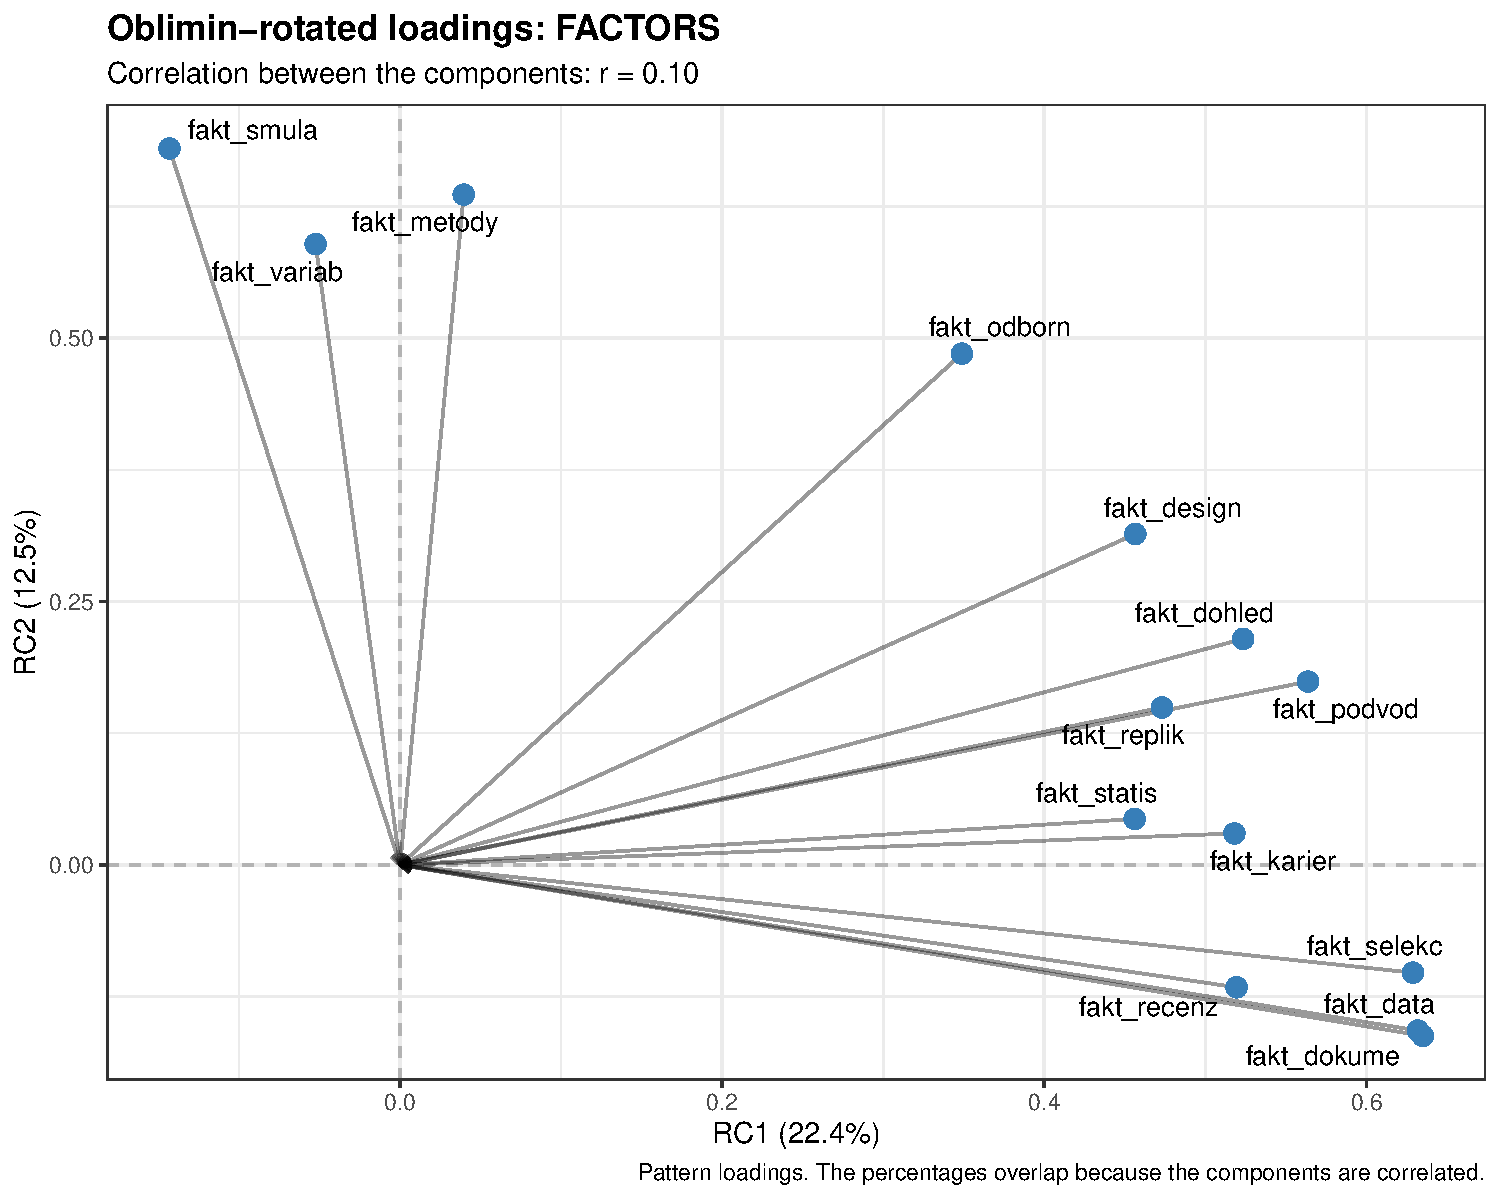
\includegraphics[width=0.82\textwidth]{PCA-oblimin-FACTORS.pdf}
\caption{Oblimin pattern loadings, group FACTORS (correlation between the components $r=0.10$).}
\label{fig:obl-FACTORS}
\end{figure}

\begin{figure}[htbp]
\centering
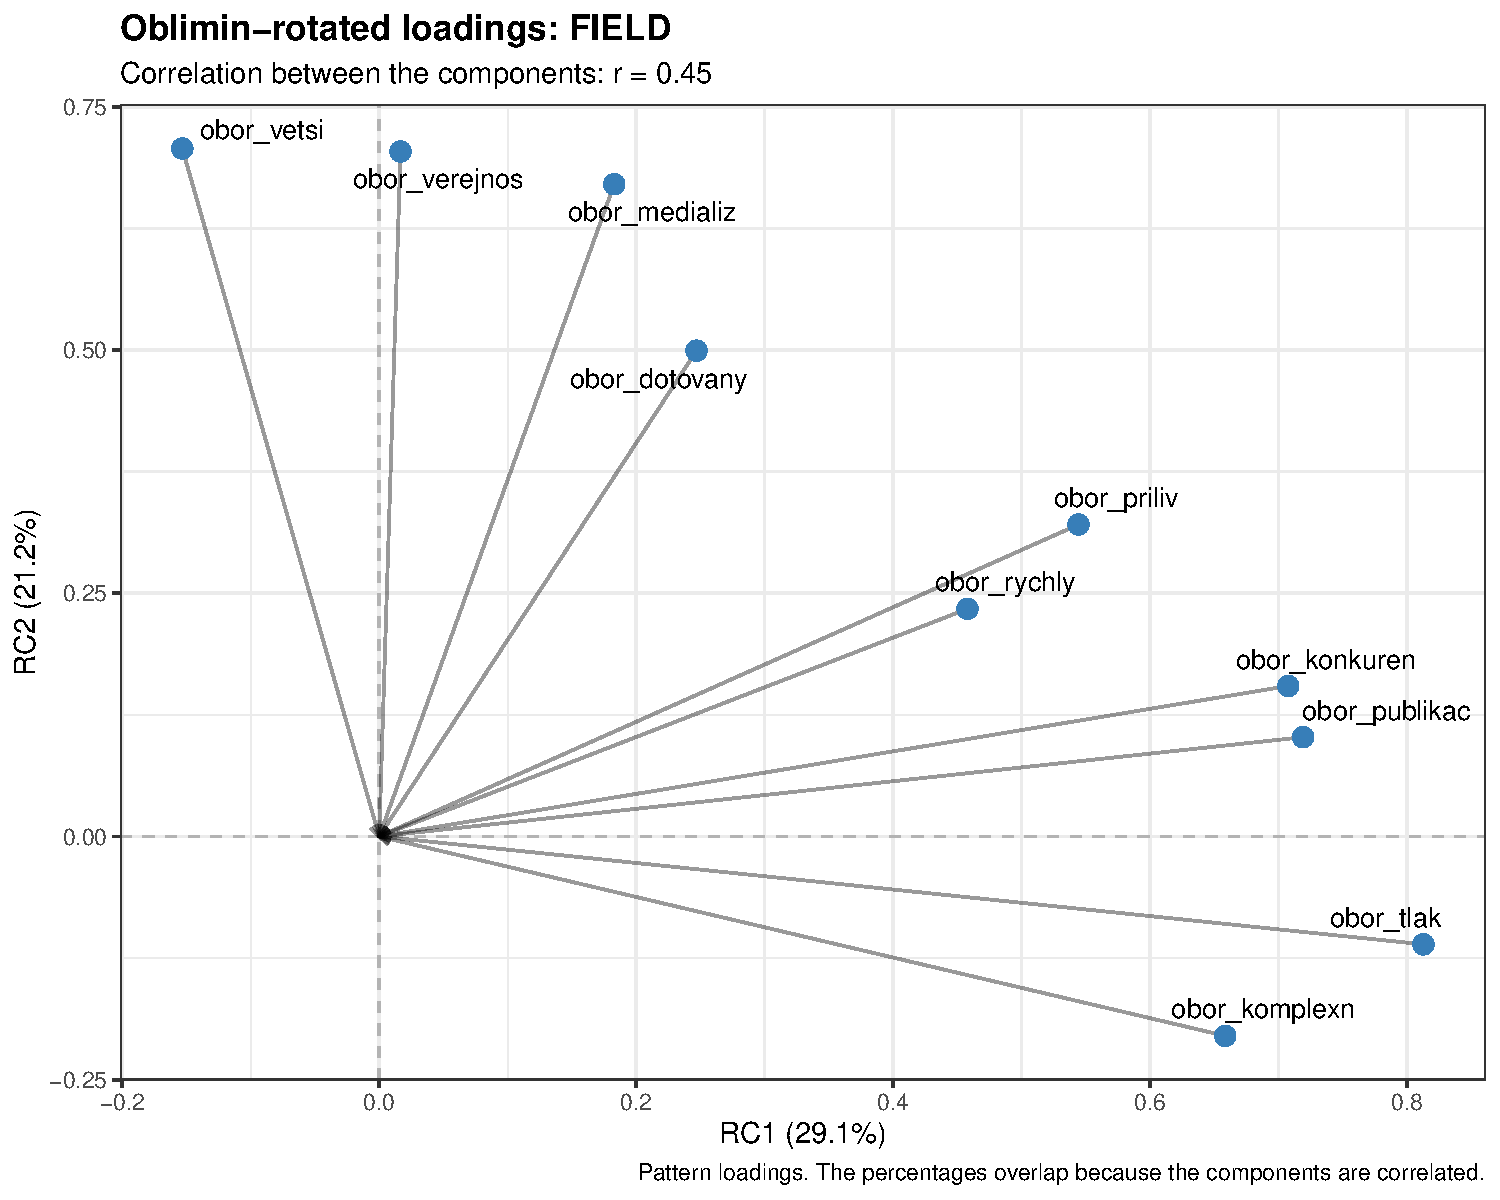
\includegraphics[width=0.82\textwidth]{PCA-oblimin-FIELD.pdf}
\caption{Oblimin pattern loadings, group FIELD ($r=0.45$).}
\label{fig:obl-FIELD}
\end{figure}

\begin{figure}[htbp]
\centering
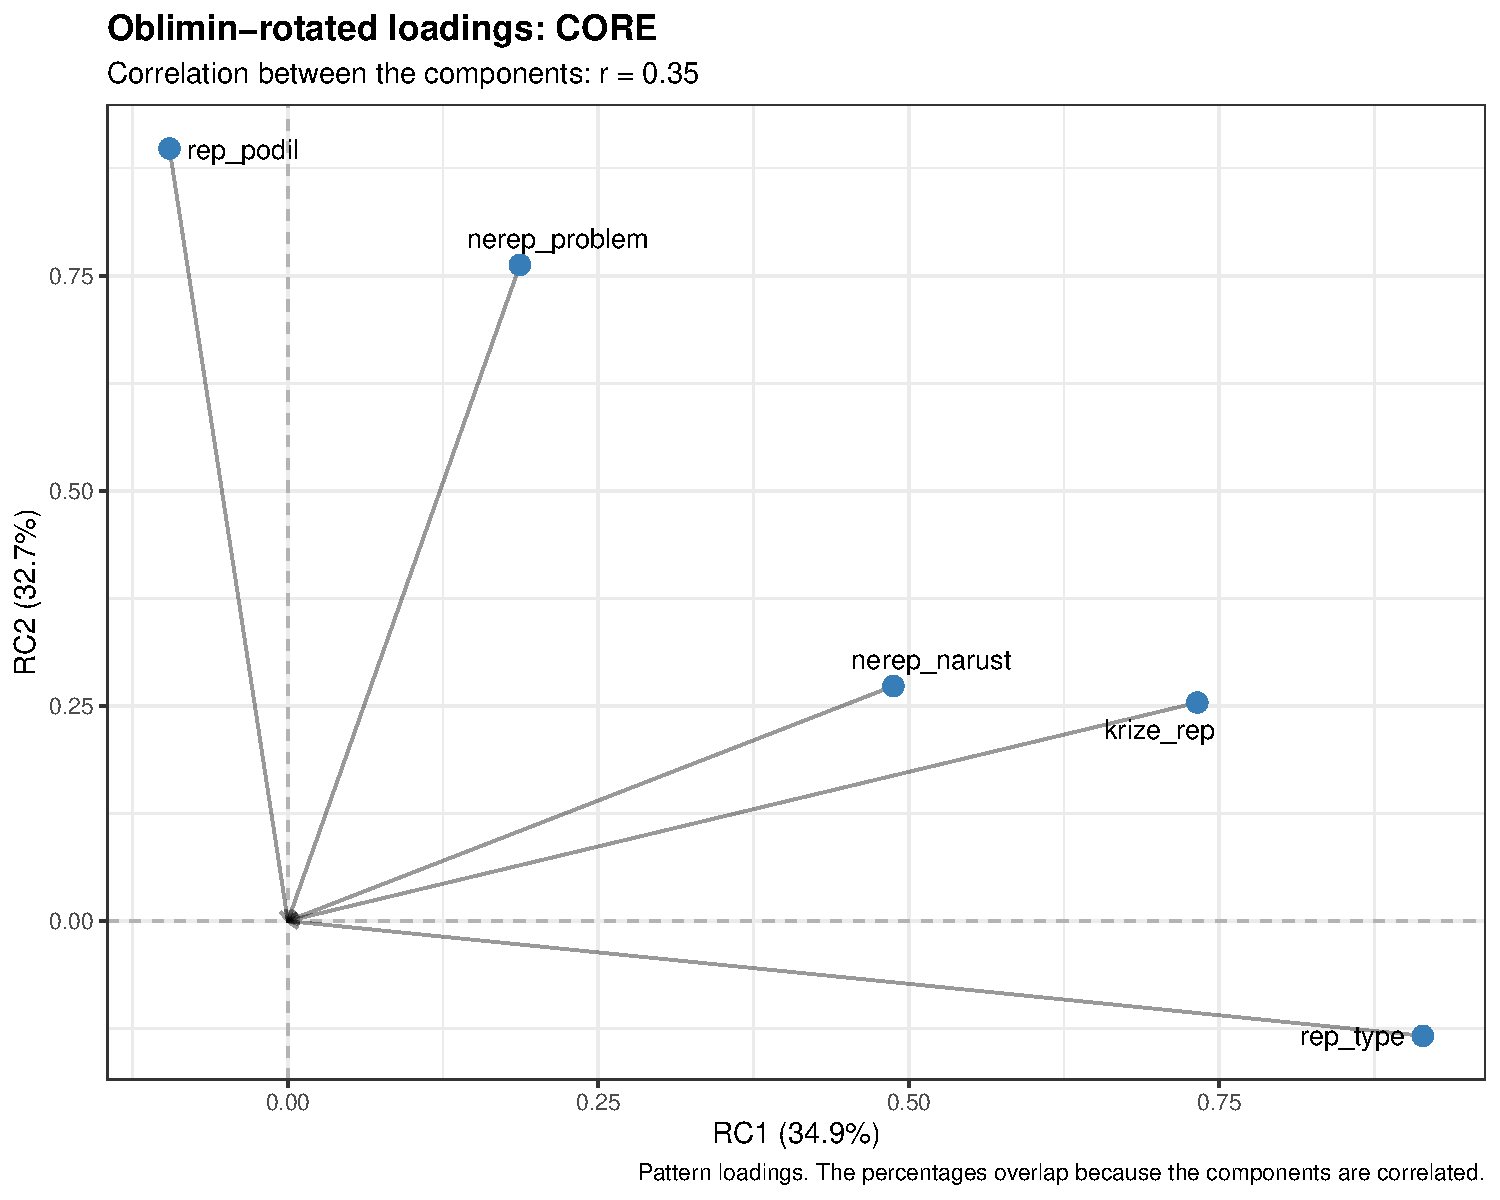
\includegraphics[width=0.82\textwidth]{PCA-oblimin-CORE.pdf}
\caption{Oblimin pattern loadings, group CORE ($r=0.35$).}
\label{fig:obl-CORE}
\end{figure}

\begin{figure}[htbp]
\centering
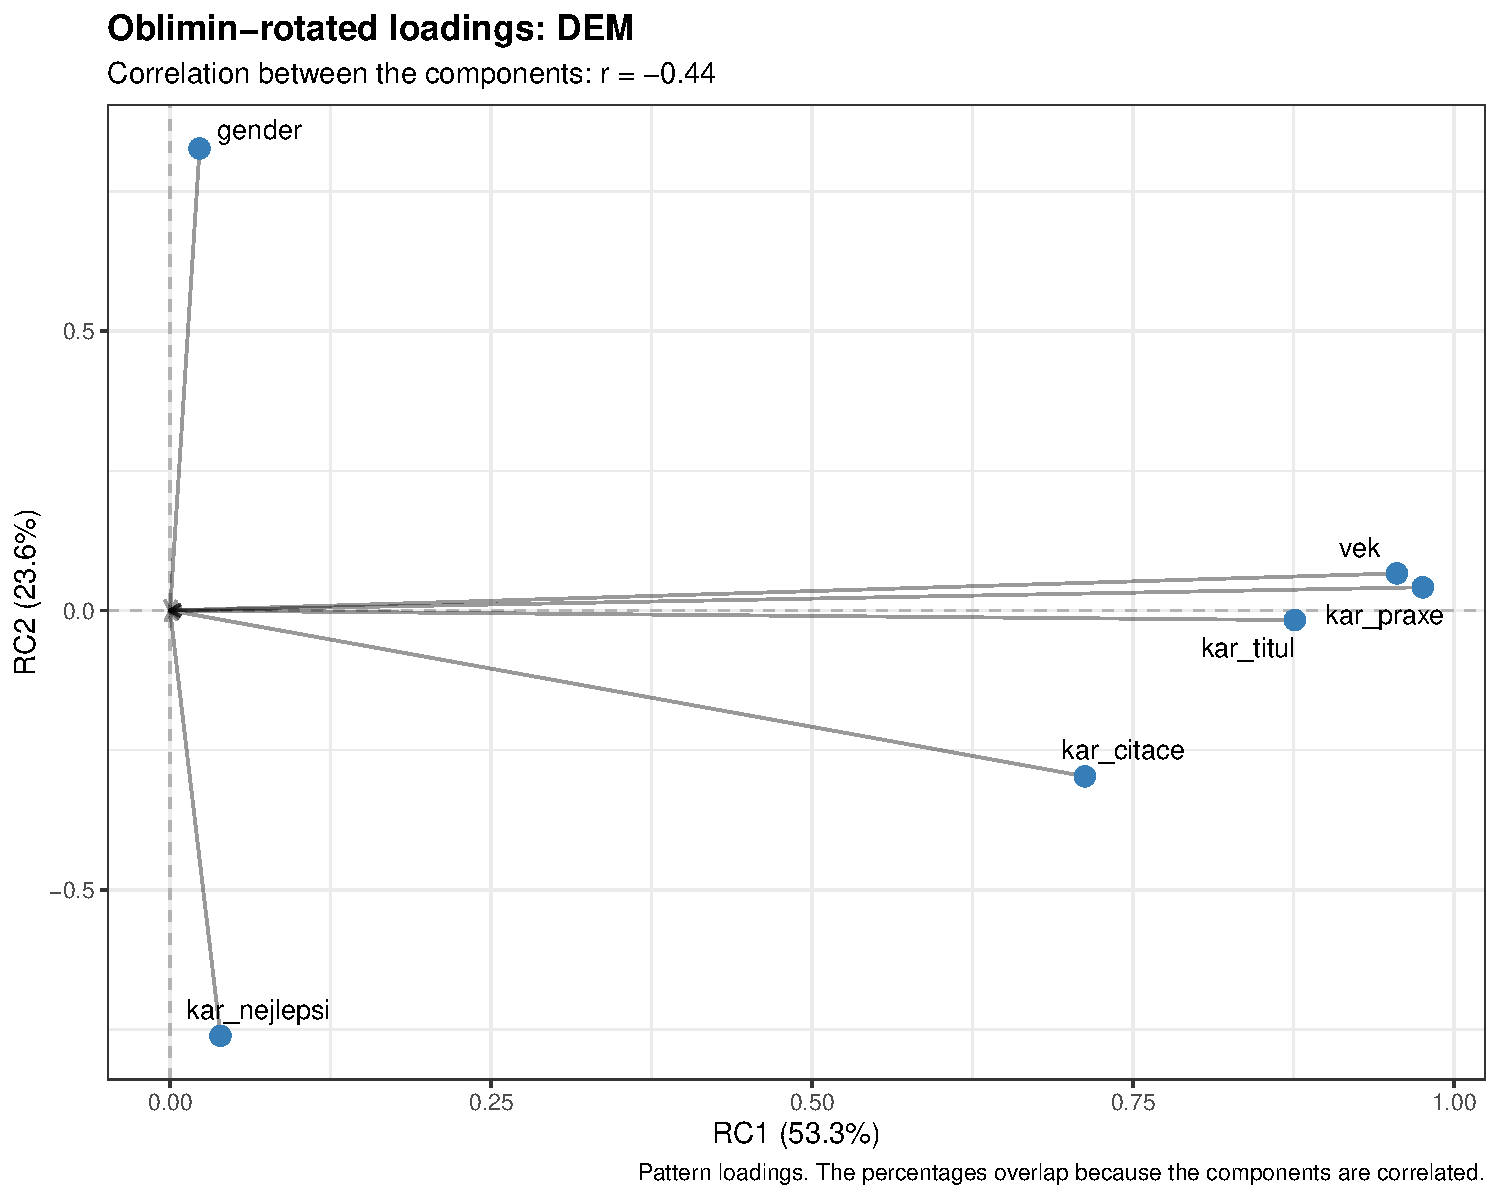
\includegraphics[width=0.82\textwidth]{PCA-oblimin-DEM.pdf}
\caption{Oblimin pattern loadings, group DEM. In this figure RC2 has the opposite sign to Appendix~\ref{app:load} (hence the printed $r=-0.44$ against $+0.44$ in Table~\ref{tab:phi}); reversing a component changes only the signs of its loadings and of its correlation with the other component.}
\label{fig:obl-DEM}
\end{figure}

\begin{figure}[htbp]
\centering
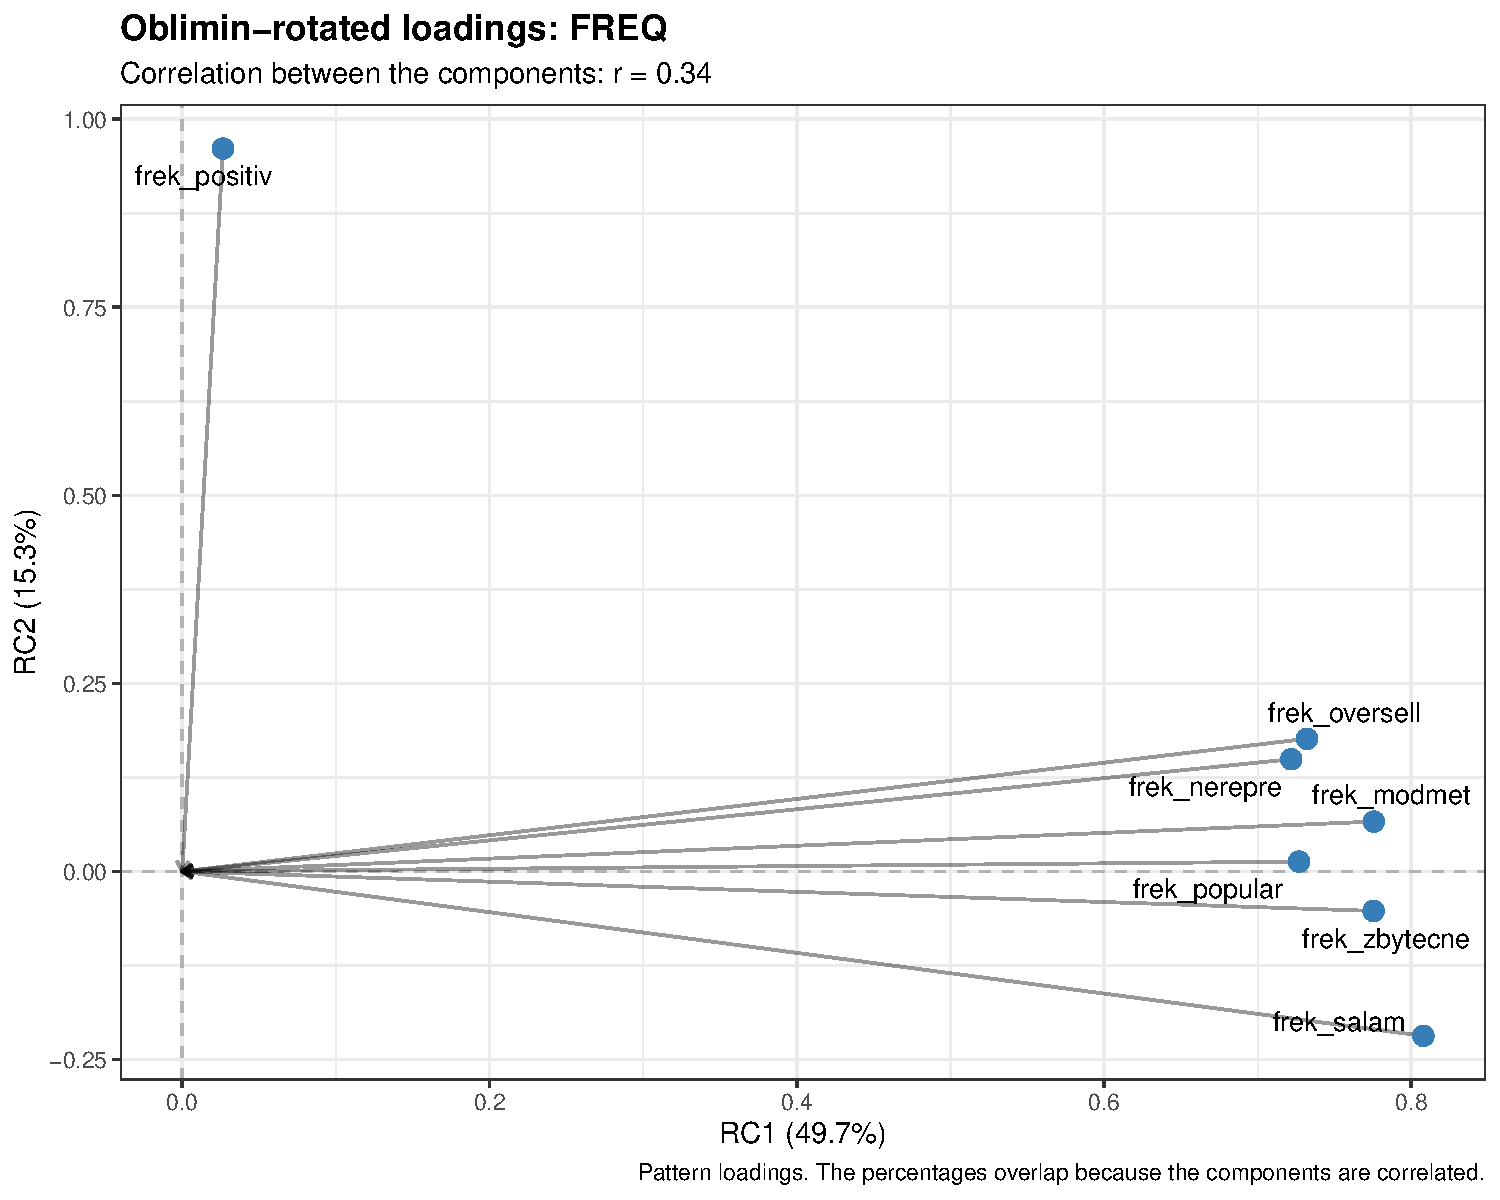
\includegraphics[width=0.82\textwidth]{PCA-oblimin-FREQ.pdf}
\caption{Oblimin pattern loadings, group FREQ ($r=0.34$).}
\label{fig:obl-FREQ}
\end{figure}

\begin{figure}[htbp]
\centering
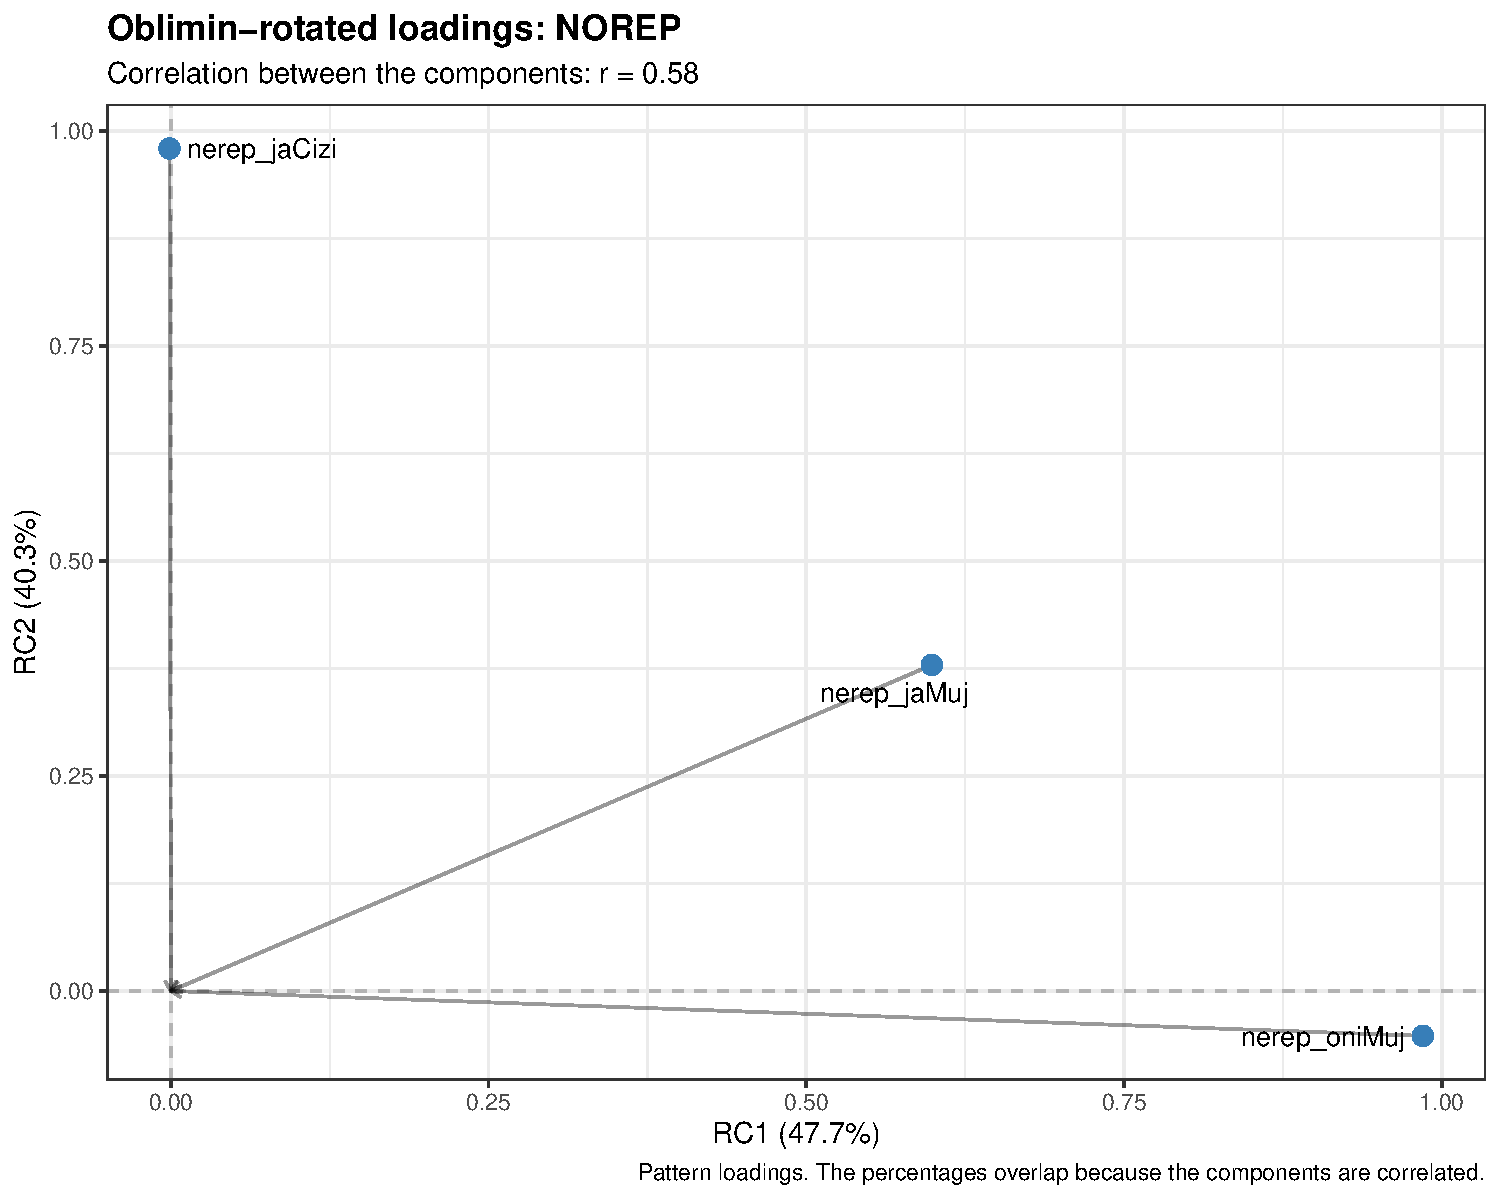
\includegraphics[width=0.82\textwidth]{PCA-oblimin-NOREP.pdf}
\caption{Oblimin pattern loadings, group NOREP ($r=0.58$).}
\label{fig:obl-NOREP}
\end{figure}

\FloatBarrier

\end{document}
